\chapter{Конструкторская часть}

\section{Требования к программному обеспечению}

\begin{enumerate}
	\item программа загружает матрицы $A$ и $B$ из текстовых файлов, пути к которым вводит пользователь; одна строка файла соответствует одной строке матрицы, элементы~--- целые числа, разделённые пробелами;
	\item при загрузке программа проверяет, что все элементы являются целыми числами, а все строки матрицы содержат одинаковое число элементов; при ошибке выводится сообщение, а ранее загруженная матрица сохраняется;
	\item перед умножением программа проверяет, что число столбцов матрицы $A$ равно числу строк матрицы $B$;
	\item программа циклически выводит меню со следующими пунктами:
	\begin{itemize}
		\item выполнение умножения выбранным алгоритмом;
		\item выполнение умножения всеми алгоритмами;
		\item вывод загруженных матриц;
		\item выбор алгоритма;
		\item загрузка матрицы $A$ из файла;
		\item загрузка матрицы $B$ из файла;
		\item замеры процессорного времени;
		\item завершение работы;
	\end{itemize}
	\item в режиме замеров программа для каждого линейного размера $N$ из набора $10, 20, \ldots, 200$ (чётные) и $11, 21, \ldots, 201$ (нечётные) генерирует случайные квадратные матрицы, выполняет их умножение каждым алгоритмом, выводит среднее процессорное время на экран и сохраняет результаты в файлы формата CSV, по одному на алгоритм.
\end{enumerate}

\section{Разработка алгоритмов}
Для каждого алгоритма определены:
\begin{itemize}
	\item $a$~--- матрица $A$ размера $n \times m$;
	\item $b$~--- матрица $B$ размера $m \times q$;
	\item $c$~--- результирующая матрица размера $n \times q$, изначально заполненная нулями.
\end{itemize}

Для алгоритмов Винограда дополнительно определены:
\begin{itemize}
	\item $mulH$~--- массив из $n$ элементов, вычисляемый по формуле~\eqref{eq:mulH};
	\item $mulV$~--- массив из $q$ элементов, вычисляемый по формуле~\eqref{eq:mulV}.
\end{itemize}

% Схемы выгружаются из algo.drawio в image/algo/<алгоритм>/<лист>.pdf скриптом export-algo.sh

\subsection{Стандартный алгоритм умножения матриц}
Схема стандартного алгоритма умножения матриц приведена на рисунке~\ref{img:standard}.

\begin{figure}[H]
	\centering
	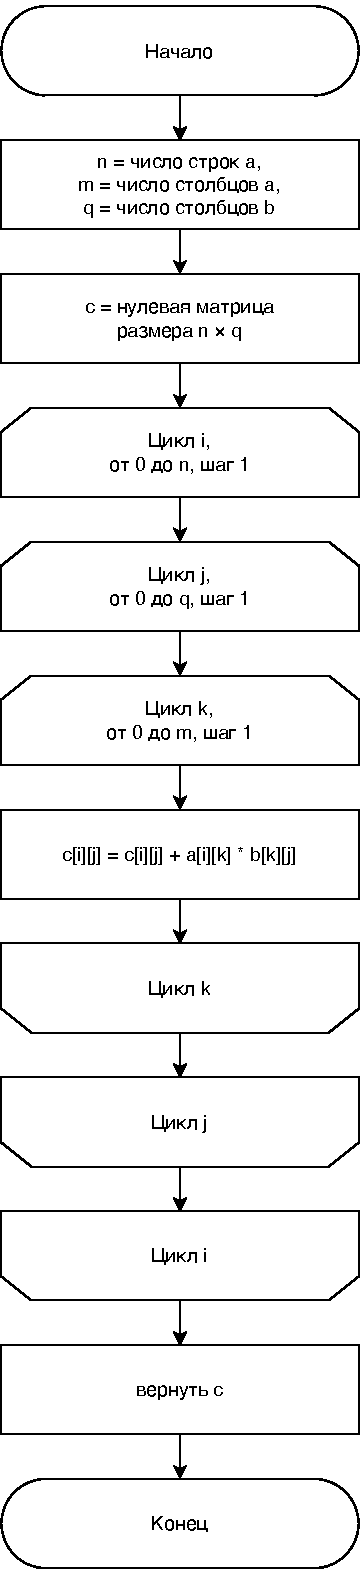
\includegraphics[scale=0.82]{image/algo/standard/1.pdf}
	\caption{Схема стандартного алгоритма умножения матриц}
	\label{img:standard}
\end{figure}

\subsection{Алгоритм Винограда}
Алгоритм состоит из четырёх этапов: вычисление массива $mulH$, вычисление массива $mulV$, вычисление элементов результата по формуле~\eqref{eq:wino-c} и добавление слагаемого $a_{i,m-1} \cdot b_{m-1,j}$ при нечётном $m$. Схема алгоритма Винограда приведена на рисунках~\ref{img:winograd-1}--\ref{img:winograd-3}.

\begin{figure}[H]
	\centering
	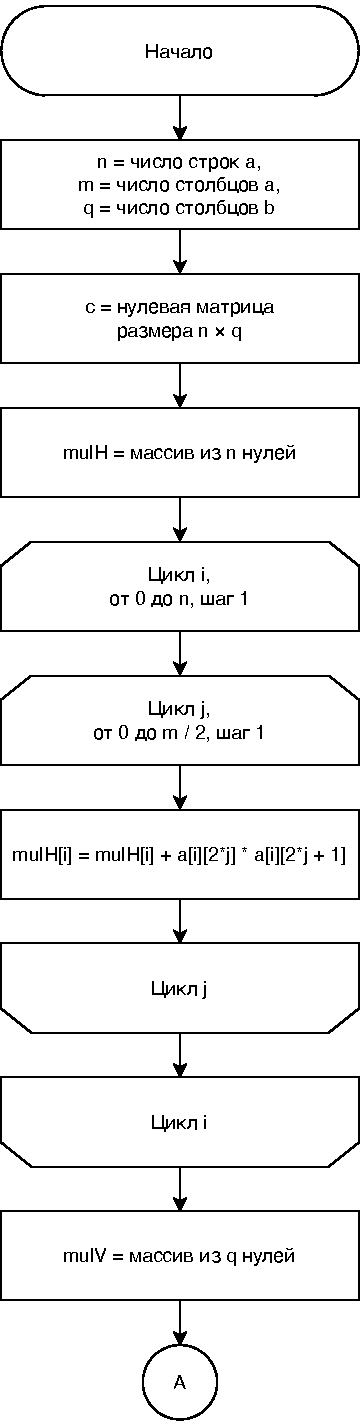
\includegraphics[scale=0.82]{image/algo/winograd/1.pdf}
	\caption{Схема алгоритма Винограда, лист 1}
	\label{img:winograd-1}
\end{figure}

\begin{figure}[H]
	\centering
	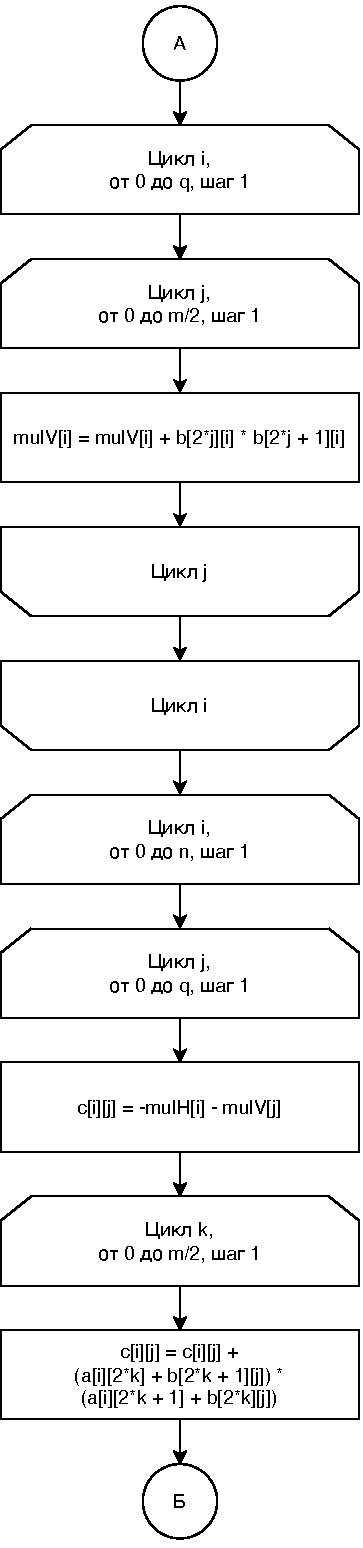
\includegraphics[scale=0.82]{image/algo/winograd/2.pdf}
	\caption{Схема алгоритма Винограда, лист 2}
	\label{img:winograd-2}
\end{figure}

\begin{figure}[H]
	\centering
	\includegraphics[scale=0.82]{image/algo/winograd/3.pdf}
	\caption{Схема алгоритма Винограда, лист 3}
	\label{img:winograd-3}
\end{figure}

\subsection{Оптимизированный алгоритм Винограда}
Согласно варианту к алгоритму Винограда применяются две оптимизации:
\begin{itemize}
	\item оптимизация А~--- деление на 2 при вычислении границы циклов по индексу пары заменяется побитовым сдвигом вправо на 1 разряд;
	\item оптимизация Б~--- накопление сумм вида $x = x + y$ заменяется составным оператором присваивания $x \mathrel{+}= y$.
\end{itemize}

Оптимизации применяются к алгоритму Винограда как по отдельности, так и совместно, что даёт три оптимизированные реализации.

\subsubsection{Реализация с оптимизацией А}
В данной реализации граница циклов по индексу пары $m / 2$ вычисляется побитовым сдвигом вправо $m \gg 1$: для неотрицательного целого $m$ оба выражения дают одинаковый результат. Сдвиг применяется во всех трёх циклах по индексу пары: при вычислении $mulH$, $mulV$ и в основном цикле. Схема алгоритма приведена на рисунках~\ref{img:winograd-shift-1}--\ref{img:winograd-shift-3}.

\begin{figure}[H]
	\centering
	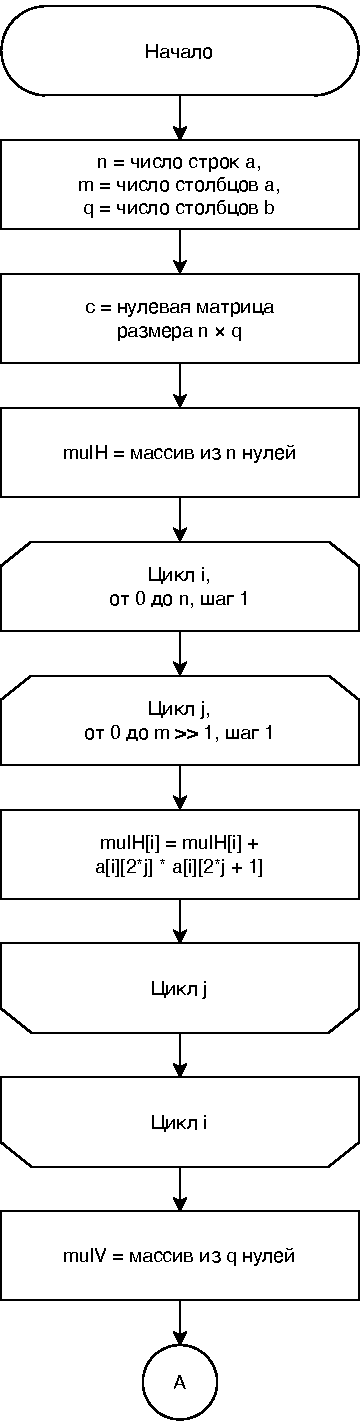
\includegraphics[scale=0.82]{image/algo/winograd-shift/1.pdf}
	\caption{Схема алгоритма Винограда с оптимизацией А, лист 1}
	\label{img:winograd-shift-1}
\end{figure}

\begin{figure}[H]
	\centering
	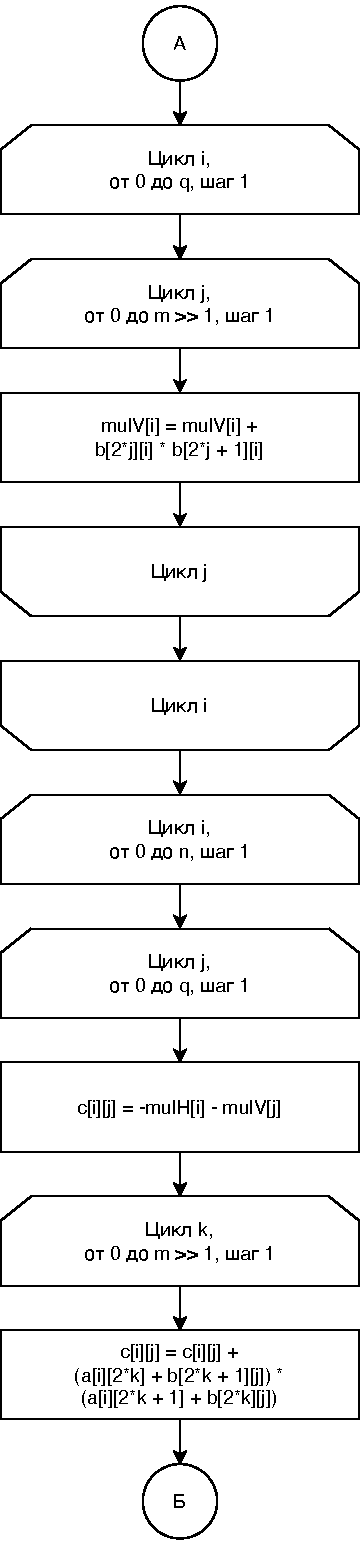
\includegraphics[scale=0.82]{image/algo/winograd-shift/2.pdf}
	\caption{Схема алгоритма Винограда с оптимизацией А, лист 2}
	\label{img:winograd-shift-2}
\end{figure}

\begin{figure}[H]
	\centering
	\includegraphics[scale=0.82]{image/algo/winograd-shift/3.pdf}
	\caption{Схема алгоритма Винограда с оптимизацией А, лист 3}
	\label{img:winograd-shift-3}
\end{figure}

\subsubsection{Реализация с оптимизацией Б}
В данной реализации все накопления сумм вида $x = x + y$ заменены составным оператором присваивания $x \mathrel{+}= y$: при вычислении $mulH$ и $mulV$, в основном цикле и при добавлении слагаемого для нечётного $m$. Это избавляет от повторного обращения к накапливаемому элементу массива в правой части присваивания. Схема алгоритма приведена на рисунках~\ref{img:winograd-add-1}--\ref{img:winograd-add-3}.

\begin{figure}[H]
	\centering
	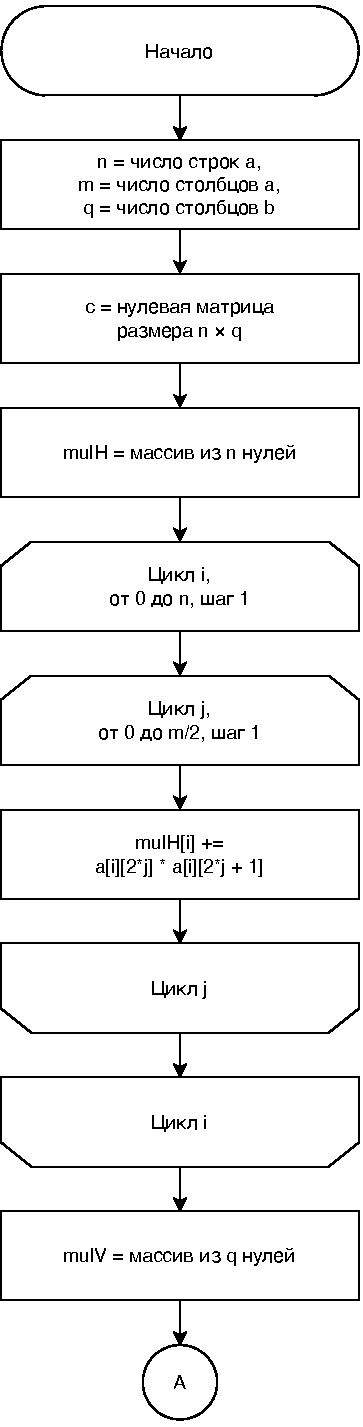
\includegraphics[scale=0.82]{image/algo/winograd-add/1.pdf}
	\caption{Схема алгоритма Винограда с оптимизацией Б, лист 1}
	\label{img:winograd-add-1}
\end{figure}

\begin{figure}[H]
	\centering
	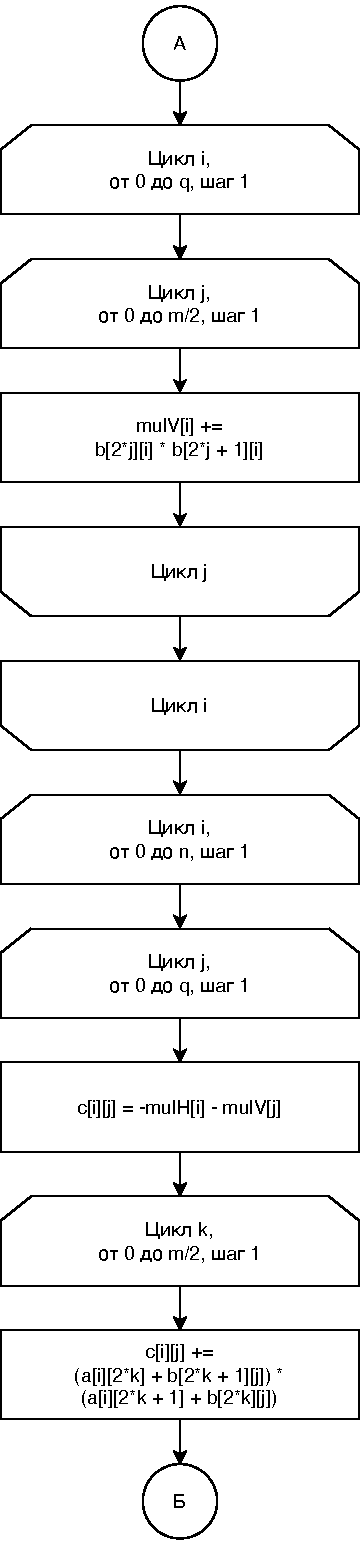
\includegraphics[scale=0.82]{image/algo/winograd-add/2.pdf}
	\caption{Схема алгоритма Винограда с оптимизацией Б, лист 2}
	\label{img:winograd-add-2}
\end{figure}

\begin{figure}[H]
	\centering
	\includegraphics[scale=0.82]{image/algo/winograd-add/3.pdf}
	\caption{Схема алгоритма Винограда с оптимизацией Б, лист 3}
	\label{img:winograd-add-3}
\end{figure}

\subsubsection{Реализация с оптимизациями А и Б}
В данной реализации обе оптимизации применяются совместно: граница циклов по индексу пары вычисляется побитовым сдвигом $m \gg 1$, а все накопления сумм выполняются составным оператором присваивания $x \mathrel{+}= y$. Схема алгоритма приведена на рисунках~\ref{img:winograd-shift-add-1}--\ref{img:winograd-shift-add-3}.

\begin{figure}[H]
	\centering
	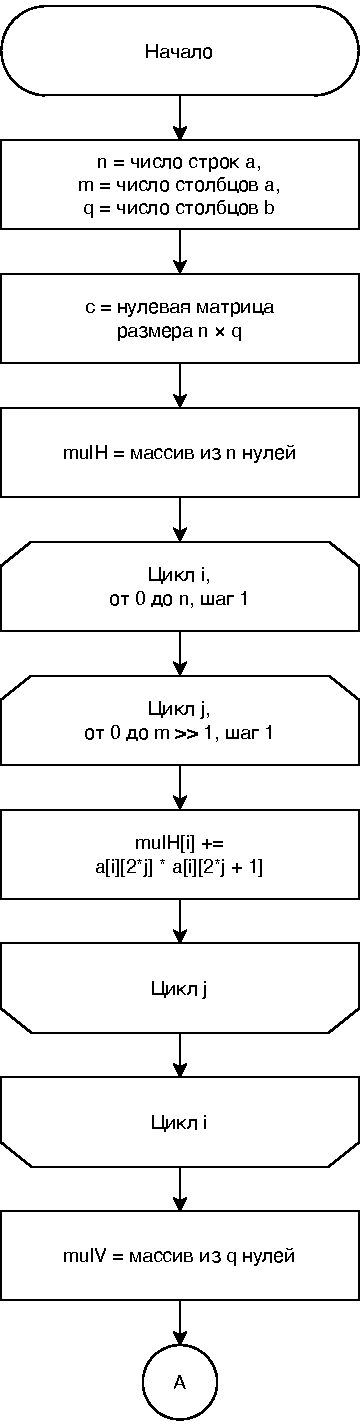
\includegraphics[scale=0.82]{image/algo/winograd-shift-add/1.pdf}
	\caption{Схема алгоритма Винограда с оптимизациями А и Б, лист 1}
	\label{img:winograd-shift-add-1}
\end{figure}

\begin{figure}[H]
	\centering
	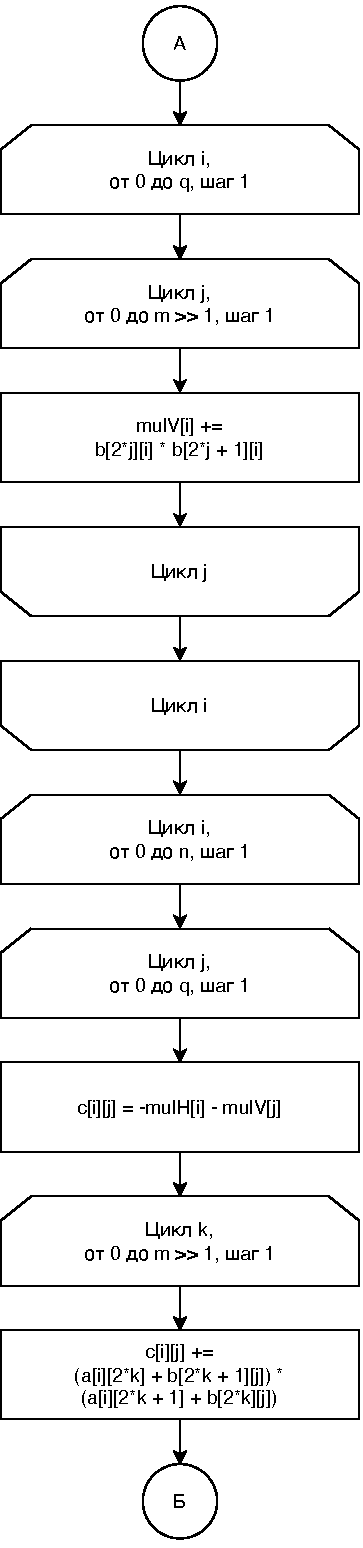
\includegraphics[scale=0.82]{image/algo/winograd-shift-add/2.pdf}
	\caption{Схема алгоритма Винограда с оптимизациями А и Б, лист 2}
	\label{img:winograd-shift-add-2}
\end{figure}

\begin{figure}[H]
	\centering
	\includegraphics[scale=0.82]{image/algo/winograd-shift-add/3.pdf}
	\caption{Схема алгоритма Винограда с оптимизациями А и Б, лист 3}
	\label{img:winograd-shift-add-3}
\end{figure}
